%===================================================================
%% H A U P T D A T E I
%%
%%
%%  Projekt: Masterarbeit 
%%  Autor:   Christof Kary
%%  Status:  
%%  Datum:   2018-04-03
%% 
%===================================================================
%% P R Ä A M B E L
%-------------------------------------------------------------------
%

\documentclass[a4paper,twoside,11pt,BCOR14mm]{scrbook}

%-------------------------------------------------------------------
%  Laden sämtlicher Packages	
%-------------------------------------------------------------------
%

\usepackage[utf8]{inputenc} % Eingabecoidierung der Umlaute nach UTF-8

\usepackage[T1]{fontenc}	% Schriftcodierung der Umlaute in westeuropäischer Form

\usepackage[ngerman]{babel}	% Neue deutsche Rechtschreibung

\usepackage{lmodern}		% Standard-Schriftfamilie Latin Modern

\usepackage{parskip}		% Absatztrennung nach europäischer Norm

\usepackage{makeidx}		% Indexerstellung

\usepackage{lipsum}			% Lorem Ipsum

\usepackage{graphicx}		% Einbetten von Grafiken
\usepackage{epstopdf} 

%\usepackage[hidelinks]{hyperref}		% Hyperlinks innerhalb des Dokumentes

\usepackage{longtable}		% Für Tabellen, die sich über mehrere Seiten erstrecken

%\usepackage{natbib}
%\bibliographystyle{unsrt}

\usepackage{url}
\usepackage[isbn=false, doi=false, backend=bibtex, sorting=none]{biblatex}
\setlength\bibitemsep{0.5\baselineskip}
\DefineBibliographyStrings{german}{% 
	urlseen = {geprüft am}, 
}
%\nocite{*}
\addbibresource{005_bib/literatur9.bib}


\usepackage{amsmath}
\usepackage{amssymb}

\usepackage[printonlyused]{acronym}

\usepackage{geometry}

\usepackage{booktabs}

\usepackage{tabulary}		% Für schönere Tabellen mit bestimmter Breite
\usepackage{colortbl}		% Für farbig hilterlegte Zellen in einer Tabelle

\usepackage{textcomp}

\usepackage{pdfpages}		%zum Einbinden von pdf-Dokumenten

\usepackage[colorlinks=true, linkcolor=black, pdfdisplaydoctitle=true,citecolor=black]{hyperref} %für pdf-Metadaten
\hypersetup{
	pdftitle    = {Weiterentwicklung eines autonom fahrenden Demonstrators für Fahrerassistenzsysteme},
	pdfsubject  = {Masterthesis},
	pdfauthor   = {Christof Kary},
	pdfpagemode  = UseOutlines, % Anzeige Bookmarks
	bookmarksopen = true,     % Anzeige Ebenen
	bookmarksnumbered = false, % Anzeige Abschnittsnummern  
	pdfstartpage = {1},        % Startseite, hilfreich mit pdf
	urlcolor=black
}

\usepackage{tikz}
\usetikzlibrary{shapes, arrows, decorations, decorations.text, decorations.pathmorphing}
\usepackage{tikz-uml} % Für UML-Diagramme
\usepackage{pgfplots} % zur Erstellung von Diagrammen

\usepackage{comment}

\usepackage{chngcntr} % Für Fußnotenummerierung global über Kapitel hinweg
\counterwithout{footnote}{chapter} 

\usepackage{svg}	% Für Bilder im .svg-Format

\usepackage{paralist} % Für Listings mit einfachem Zeilenabstand

\usepackage{todonotes} % Um Bilder und Grafiken auszublenden und Platzhalter zu verweden

\usepackage[decimalsymbol=comma,loctolang={DE:ngerman,UK:english}]{siunitx} % Für SI-Einheiten

%-------------------------------------------------------------------
%  Pfade der Dateien setzen
%-------------------------------------------------------------------
%
\graphicspath{{006_img/}}

%-------------------------------------------------------------------
%  Sonstige Befehle	
%-------------------------------------------------------------------
%
\makeindex

\linespread{1.1} % Zeilenabstand für Dokument % Einfügen der Präambel aus der Header-Datei

%===================================================================
% B E G I N N  D E S  D O K U M E N T S
%-------------------------------------------------------------------

\begin{document}

%-------------------------------------------------------------------
%  VORSPANN	
%-------------------------------------------------------------------
%
	% Die folgenden Seiten besitzen keine Seitennummerierung
	\renewcommand{\maketitle}{%

\begin{titlepage}
	\thispagestyle{empty}
	\oddsidemargin14mm
	\evensidemargin4mm
	\centering
	\begin{center}
		

		
\includegraphics[height=2cm]{01_deckblatt/hska_cmyk_claim_II-goem.eps} \hfill
		
\includegraphics[height=2cm]{01_deckblatt/Evomotiv_logo}\\ 
		
		\vspace{2em}
		
		\large{Hochschule Karlsruhe -- Technik und Wirtschaft \\ Fakultät für Maschinenbau und Mechatronik}\\
		
		\vspace{10mm}
	
		\textsf{
		{\huge  \bfseries Weiterentwicklung eines autonom fahrenden Demonstrators für Fahrerassistenzsysteme\\}}
		%
		\vspace{15mm}
		%    
		\large{Thesis \\zur Erlangung des Grades \\ \vspace{1ex}
		\bfseries Master of Science (M.~Sc.)}
		%    
		\vspace{15mm}\\
		Christof Kary\\
		geb. am 05.04.1993\\
		in Rastatt\\
		Matrikel-Nr.: 58516\\
		
		\vspace{15mm}
		Betreuer der Hochschule Karlsruhe\\
		Herr Prof. Dr.-Ing. Ferdinand Olawsky\\
		\vspace{1em}
		Betreuer am Arbeitsplatz\\
		Herr Dipl.-Ing. (FH) Arthur Kessler\\
		
		\vspace{10mm}
		Flacht, 1. April 2018 bis 30. September 2018\\

		%
	\end{center}

\end{titlepage}
}


\maketitle
		% Deckblatt an erster Seite einfügen
	
	\chapter*{Aufgabenbeschreibung}
\thispagestyle{empty}	% Aufgabenbeschreibung
	
	\chapter*{Eidesstattliche Erklärung}
\thispagestyle{empty}

Der Verfasser erklärt, dass er die vorliegende Arbeit selbständig, ohne fremde Hilfe und ohne Benutzung anderer als der angegebenen Hilfsmittel angefertigt hat. Die aus fremden Quellen (einschließlich elektronischer Quellen) direkt oder indirekt übernommenen Gedanken sind ausnahmslos als solche kenntlich gemacht. Die Arbeit ist in gleicher oder ähnlicher Form oder auszugsweise im Rahmen einer anderen Prüfung noch nicht vorgelegt worden.\\

\vspace{10mm}
	
	\begin{center}
		
		\begin{tabular}{l l}
			Flacht, den \today \hspace{20mm} & \hspace{60mm} \\ \cline{2-2} 
			                                 & \\
			                                 & Christof Kary
		\end{tabular}
	\end{center}

\vspace{10mm}

 	% Eidesstattliche Erklärung
	
	\chapter*{Vorwort}
\thispagestyle{empty}

Danksagung\\
\newline
\lipsum[1-2]
		% Vorwort mit Danksagung
	
	
	\frontmatter	% Hier beginnt Seitennummerierung in römisch groß
	\pagenumbering{Roman}  
	\chapter{Kurzfassung} \label{vor:kurzfassung}

\textsf{\Large \bfseries Titel der Arbeit in deutscher Sprache}

\lipsum[1-2]

	
	\chapter{Abstract} \label{vor:abstract}

\textsf{\Large \bfseries Titel der Arbeit in englischer Sprache}

\lipsum[1-2]

	
	\chapter{Abkürzungsverzeichnis} \label{vor:abkuerzungsverzeichnis}

% \manualmark
% \markright{Abkürzungsverzeichnis}
% \markleft{Abkürzungsverzeichnis}

% ACHTUNG: Muss von Hand alphateisch sortiert werden!

\renewcommand{\arraystretch}{1.25} % Zeilenhöhe auf Faktor 1.25 erhöhen

\textbf{\textsf{Kurzform}} \hspace{2.5cm} \textbf{\textsf{Bedeutung}}
\vspace{1ex}

\setlength{\itemsep}{-\parsep}	% Ausrichtung am längsten Akronym
\begin{acronym}[MMMMMMMMMM]		% länsgtes Akronym
	\acro{muc}[$\mu$C]{Mikrocontroller}
	\acro{ACK}{Acknowledgement}
	\acro{Bus}{Binary Utility System}
	\acro{CAN}{Controller Area Network}
	\acro{CAPL}{Communication Access Programming Language}
	\acro{CRC}{Cyclic Redundancy Check}
	\acro{CSMA/CA}{Carrier Sense Multiple Access with Collision Avoidance}
	\acro{ECU}{Electronic Control Unit}
	\acro{HSKA}{Hochschule Karlsruhe – Technik und Wirtschaft}
	\acro{ID}{Identifier}
	\acro{ISO}{International Organization for Standardization}
	\acro{KWP}{Keyword Protokoll}
	\acro{LIN}{Local Interconnect Network}
	\acro{MOST}{Media Oriented Systems Transport}
	\acro{OBD}{On-Board-Diagnose}
	\acro{OSI}{Open System Interconnection}
	\acro{SG}{Steuergerät}
	\acro{UDS}{Unified Diagnostic Services}
	\acro{UML}{Unified Modeling Language}
	
\end{acronym}

\renewcommand{\arraystretch}{1} % Zeilenhöhe auf Standard zurücksetzen

	
	\chapter{Nomenklatur} \label{vor:nomenklatur}

% \manualmark
% \markright{Nomenklatur}
% \markleft{Nomenklatur}

\renewcommand{\arraystretch}{1.25} % Zeilenhöhe auf Faktor 1.25 erhöhen
\begin{longtable}{p{0.2\textwidth} p{0.2\textwidth} p{0.6\textwidth}}
	\textbf{\textsf{Zeichen}} & \textbf{\textsf{Einheit}} & \textbf{\textsf{Dimension}} \vspace{1ex} \\
	$\vartheta$               & C                         & Temperatur 	\\
	$\varrho$                 & kg/m$^3$                  & Dichte		\\
	$p$                       & N/m$^2$                   & Druck
\end{longtable}
\renewcommand{\arraystretch}{1} % Zeilenhöhe auf Standard zurücksetzen
	
	\tableofcontents
	
%-------------------------------------------------------------------
%  EINLEITUNG
%-------------------------------------------------------------------
%
	\mainmatter
	
	\chapter{Einleitung} \label{cha:einleitung}

\section{Motivation} \label{sec:motivation}
Bereits seit einigen Jahren zeichnet sich durch den Einzug moderner Fahrerassistenzsysteme ein Umbruch im individuellen und gesellschaftlichen Umgang mit dem Automobil ab. Als treibende Aspekte für den technologischen Umbruch in der Automobilentwicklung sind die steigende Verkehrssicherheit, der erhöhte Fahrkomfort und eine energieoptimale Fahrzeugführung zu nennen. Alleine im Jahr 2017 kamen 3.177 Menschen bei Verkehrsunfällen auf deutschen Straßen ums Leben [Quelle].
FAS bieten Potential um Unfälle zu senken. 

Autonomes Fahren könnte einen Umbruch im individuellen und gesellschaftlichen Umgang
mit dem Automobil nach sich ziehen und damit auch Einfluss nehmen auf Verkehr,
Mobilität oder Raumstrukturen.

\section{Zielsetzung der Arbeit} \label{sec:aufgabenstellung}
\lipsum[1-3]
	
	\chapter{Grundlagen} \label{cha:grundlagen}
Die vorliegende Schrift ist grundsätzlich als Forschung- und Entwicklungsarbeit des automatisierten Fahrens in der Automobilbranche anzusiedeln. Es werden zunächst einige Schlüsseltechnologien der Fahrerassistenzsysteme vorgestellt und Ihre Notwendigkeit für den Entwicklungsfortschritt hin zum vollautomatisierten Fahren begründet.


\section{Autonomes Fahren} \label{sec:AutonomesFahren}
% Unterschied automatisiertes/autonomes Fahren

\subsection{Überblick Fahrerassistenzsysteme} \label{subsec:FAS}
\lipsum[1-1]
\subsection{Autonomiestufen} \label{Autonomiestufen}% 5-Stufen des autonomen Fahrens
\lipsum[1-1]


\section{Bussysteme} \label{sec:Bussysteme}
Die rasante Zunahme an elektronischen Systemen und \emph{Steuergeräten} \acs{SG} (englisch \emph{\acl{ECU}} \acs{ECU}) in den letzten Jahrzehnten machten einen geregelten Datenaustausch in der Fahrzeugtechnik unerlässlich. Stetig steigende Anforderungen an Fahrsicherheit, Motorsteuerung und Komfortsysteme erforderten zwingend einen sicheren und schnellen Informationsfluss zwischen den kommunizierenden Steuergeräten, sodass ein verteiltes und vernetztes Gesamtsystem entstand. Alle für eine jeweilige Funktion benötigten Daten konnten systemweit zur Verfügung gestellt werden. Aus dem zunehmenden Elektrifizierungsgrad ergaben sich heutige moderne Elektronikarchitekturen im Kfz in Form von seriellen Bussystemen. Das Akronym \acs{Bus} stammt \cite{Klumann.2000} nach von \emph{\acl{Bus}}, was auf ein drahtgebundenes Übertragungsmedium mit Anschluss an alle Systemkomponenten hinweist. Es werden komplexe Datenmengen über einzelne Leitungen bitweise übertragen, wodurch sich eine Vielzahl an Vorteilen ergibt: Der Verkabelungsaufwand sämtlicher elektrischer Leitungen wird minimiert, wodurch sich die Kosten, das Gewicht und die Fehleranfälligkeit reduzieren. Zudem wird eine Mehrfachnutzung von Informationen möglich, was die Anzahl der verbauten Sensoren senkt. Eine Diagnosefunktion wird umsetzbar und das Gesamtsystem ist flexibel für Änderungen und Erweiterungen. Die Kommunikation innerhalb eines Gesamtsystems, welches aus mehreren miteinander verknüpften Bussystemen bestehen kann, wird als \emph{On-Board-Kommunikation} bezeichnet. Um eine übergeordnete Datenkommunikation einzelner Vernetzungsbereiche und Netzwerke zu erhalten, müssen die einzelnen Bussysteme mit unterschiedlichen Protokollen physikalisch und logisch miteinander verbunden werden. Diese Funktion wird von einem \emph{Gateway} übernommen. Ein Gateway stellt sämtliche Daten netzwerkübergreifend zur Verfügung. Dabei kann die Funktion entweder in bereits vorhandene Steuergeräte integriert werden oder es kommen eigene zentrale oder dezentrale Gateway-Steuergeräte zum Einsatz. Bei einer \emph{Off-Board-Kommunikation} stellt ein Gateway die Verbindung zwischen dem geschlossenen Gesamtnetz im Fahrzeug zu einem externen Gerät her \cite{VectorInformatikGmbH.b}. \\

Heute standardisierte und gängige Datenkommunikationssysteme sind in Tabelle \ref{tab:KlassifikationSerielleBussysteme} aufgeführt \cite{VectorInformatikGmbH.b}. Auf die zur Anwendung wichtigste Form der Buskommunikation, dem \emph{\acs{CAN}-Bus}, wird an späterer Stelle näher eingegangen. \\
Neben dem heutzutage am häufigsten eingesetzten Bussystem (vgl. Unterabschnitt \ref{subsec:CAN}) haben sich aufgrund der speziellen Anwendungsfälle und der Eigenentwicklung unterschiedlichster Hersteller, vor allem aber zur Kostenreduzierung, weitere Systeme etabliert. Die kostengünstige Variante zur seriellen Datenübertragung \emph{Local Interconnect Network} \acs{LIN} weist eine vergleichsweise geringe Datenrate auf und wird daher mittlerweile lediglich in der Komfortelektronik als Kommunikationsschnittstelle zwischen Sensorik und Aktorik verbaut.Da als physikalisches Übertragungsmedium nur eine Eindrahtleitung zum Einsatz kommt, ist das Netzwerk relativ störanfällig, was eine Verwendung in sicherheitsrelevanten Bereichen ausschließt. Eine deutlich höhere Ausfallsicherheit, aber zugleich signifikant teurere Datenübertragung liefert der sog. \emph{FlexRay}. Aufgrund der hohen Datenraten von bis zu 10\,Mbit/s bietet dieses deterministische Feldbussystem ein hohes Potential für zeit- und sicherheitskritische Anwendungsfälle \cite{VectorInformatikGmbH.c}. Für Multimediaanwendungen im Automobilbereich hat sich der \emph{Media Oriented Systems Transport} \acs{MOST}-Bus etabliert, der als Übertragungsmedium Lichtwellenleiter verwendet und damit sehr hohe Bitraten von bis zu 150\,Mbit/s ermöglicht Ein MOST-Netzwerk ist in der Regel als Ringtopologie aufgebaut und liefert daher eine lediglich geringe Ausfallsicherheit \cite{Schuller.20.01.2005}.\\


\begin{table}[!htbp]
	\centering
	\caption{Klassifikation serieller Bussysteme \cite{VectorInformatikGmbH.b}}
	\renewcommand{\arraystretch}{1.3}
	\begin{tabulary}{\columnwidth}{L L L L L}
		\toprule
		Bussystem        & Typische Anwendung           & Maximale Datenrate & Übertragungsmedium          & Sicherheits-anforderung \\ \midrule
		LIN              & Komfort, Karosserie          & 20 kbit/s          & Eindrahtleitung             & gering                  \\
		CAN (Low Speed)  & Komfort, Karosserie          & 125 kbit/s         & Verdrillte Zweidrahtleitung & hoch                    \\
		CAN (High Speed) & Antrieb, Fahrwerk, Diagnose  & 1 Mbit/s           & Verdrillte Zweidrahtleitung & hoch                    \\
		FlexRay          & Fahrwerk, \newline X by Wire & 10 Mbit/s          & Verdrillte Zweidrahtleitung & sehr hoch               \\
		MOST             & Infotainment                 & 150 Mbit/s         & Lichtwellenleiter           & gering                  \\ \bottomrule
	\end{tabulary}

	\label{tab:KlassifikationSerielleBussysteme}
\end{table}



\subsection{Kommunikationsmodell} \label{subsec:Kommunikationsmodell}
Um einen reibungslosen und nachvollziehbaren Datenaustausch zu gewährleisten, mussten mit dem Einzug der Bussysteme in der Automobilentwicklung auch einheitliche, herstellerübergreifende Kommunikationsstrukturen eingeführt werden. 1983 wurde der gesamte Datentransfer in einem Datennetz von der \emph{International Organization for Standardization} \acs{ISO} in sieben einzelne \emph{Layer} (Schichten) unterteilt und die komplexe Kommunikationshierarchie beschrieben. Durch das in \emph{DIN EN ISO/IEC 7498-1} \cite{InternationalOrganizationforStandardization.15.11.1994} festgehaltene \emph{Open System Interconnection} \acs{OSI}-Schichtenmodell kann eine standardisierte und herstellerübergreifende Kommunikation im gesamten Busnetzwerk erzielt werden. Das OSI-Schichtenmodell wird in Tabelle \ref{tab:OSI-Schichtenmodell} beschrieben. Für die Automobilindustrie und für Kfz-Anwendungen sind die grau hinterlegten Schichten noch nicht relevant. Wichtig sind vor allem die beiden untersten Layer \emph{Physical} und \emph{Data Link}. Diese Schichten werden an späterer Stelle genauer beschrieben. 

\begin{table}[!htbp]
	\centering
	\caption{Zusammenfassung des OSI-Schichtenmodells aufgeteilt in Layer,
		Schicht und Funktionen \cite{InternationalOrganizationforStandardization.15.11.1994}}
	\renewcommand{\arraystretch}{1.3}
	\begin{tabular}{l l l p{7.5cm}}
														  	   \toprule
		  &  Layer        & Schicht           & Funktion	\\ \midrule
		7 & Application  & Anwendung         & Zugriff auf das Kommunikationssystem, Entkopplung Anwendung von Kommunikation    		\\
		\rowcolor[gray]{.9} 6 & Presentation & Darstellung       & Semantik, Datenkompression, Verschlüsselung,
		Übersetzer verschiedener Datenformate 			\\
		\rowcolor[gray]{.9} 5 & Session      & Sitzungssteuerung & Unterhalten längerer Sitzungen, Definition von
		Synchronisationspunkten            				\\
		4 & Transport    & Datentransport    & Verbindungsauf- und -abbau, Segmentierung,
		Sequenzierung, Assemblierung            		\\
		\rowcolor[gray]{.9} 3 & Network      & Vermittlung       & Routing, Adressvergabe, Teilnehmererkennung
		und -überwachung                       			\\
		2 & Data Link    & Datensicherung    & Botschaftsaufbau, Buszugriff, Flusskontrolle
		Fehlersicherung                       			\\
		1 & Physical     & Bitübertragung    & Physikalische Busankopplung, Stecker,
		Übertragungsmedium, Leitungscodierung        	\\ \bottomrule
	\end{tabular}
	
	\label{tab:OSI-Schichtenmodell}
\end{table}


\subsection{Controller Area Network CAN} \label{subsec:CAN}
Das Bussystem \emph{Controller Area Network} \acs{CAN} wurde erstmals in den 1980er Jahren von der \emph{Robert Bosch GmbH} präsentiert und gilt seit 1994 als offener Industriestandard. Mit der \acs{ISO}-Norm \emph{ISO 11898} wurde die \acs{CAN}-Spezifikation international vereinheitlicht. Heute stellt \acs{CAN} durch seine hohe Datenübertragungsrate und der geringen Fehleranfälligkeit die am weitesten verbreitete Kommunikationsspezifikation in der Automobilindustrie dar, kommt jedoch auch häufig in industriellen Anwendungen zum Einsatz. Aufgrund der daraus resultierenden hohen Stückzahlen an \acs{CAN}-Controllern ergibt sich ein stetig sinkender Stückpreis für die zugehörigen Steuergeräte, was als weitere Stärke dieses Bussystems zu zählen ist. 
Die Steuergeräte, oder auch \emph{Bus-Knoten} bezeichnet, sind in einem \acs{CAN}-Netzwerk üblicherweise in Form einer Linientopologie nach der \emph{Multi-Master}-Architektur miteinander verbunden. Jeder Knoten ist berechtigt, den Datentransfer auf dem Bus ereignisgesteuert anzustoßen \cite{Wallentowitz.2011, Zimmermann.2014}.

\subsection{CAN-Protokoll: Physical Layer} \label{subsec:PhysicalLayer}
Die unterste Schicht im \acs{OSI}-Modell beschreibt die physikalische Busankopplung. Das Übertragungsmedium des \acs{CAN}-Busses wird in den häufigsten Fällen als verdrillte Zweidrahtleitung, als sog. \emph{Twisted-Pair-Leitung}, ausgeführt, wodurch sich die magnetischen Felder der beiden Leitungen weitestgehend gegenseitig neutralisieren. Eine hohe Datenrate und Busauslastung können zu Reflexionen im Bussystem führen. Um diesen unerwünschten Effekt zu minimieren, müssen die Enden der Busleitung mit einem Abschlusswiderstand versehen werden. Neben der physikalischen Busleitung kommen hardwareseitig weitere Bauteile wie der \emph{Mikrocontroller} (\acs{muc}), der \acs{CAN}-Controller und der \acs{CAN}-Transceiver zum Einsatz. Der Mikrocontroller verarbeitet die Kommunikationsdienste der höheren \acs{OSI}-Schichten in der Kommunikationssoftware. Die grundlegenden Funktionen sind hingegen in den restlichen Bauteilen implementiert. Der \acs{CAN}-Controller wickelt das Protokoll ab, während der Transceiver die physikalische Verbindung zum Übertragungsmedium herstellt. Der prinzipielle Aufbau eines \acs{CAN}-Netzwerks wird in Abbildung \ref{abb:CANNetzwerk} verdeutlicht.

\begin{figure}[!htbp]
	\centering
	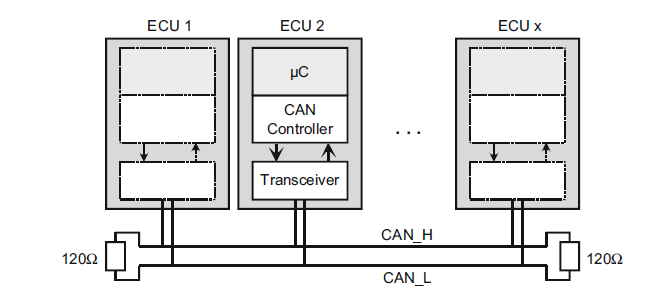
\includegraphics[width=0.8\textwidth]{./2_2_3_CAN-Netzwerk}
	\caption{CAN-Netzwerk: Ein einzelner \acs{CAN}-Knoten besteht aus einem Mikrocontroller, einem \acs{CAN}-Controller und einem \acs{CAN}-Transceiver. Der Abschlusswiderstand unterdrückt	Busreflexionen \cite{Zimmermann.2014}.}
	\label{abb:CANNetzwerk}
\end{figure}

Die physikalische Signalübertragung in einem \acs{CAN}-Netzwerk basiert auf der Übertragung von Spannungsdifferenzen zwischen der \emph{\acs{CAN}-High}-Leitung (CANH) und der \emph{\acs{CAN}-Low}-Leitung (CANL). Wie in Tabelle 2-1 dargestellt, unterscheidet die \acs{ISO}-Norm zwischen dem \emph{Low-Speed-\acs{CAN}} (Class B) und dem \emph{High-Speed-\acs{CAN}} (Class C). Der Low-Speed-\acs{CAN} zeichnet sich durch seine auf 125\,kbit/s begrenzte Datenrate aus. Dadurch findet er häufig in Komfortsystemen wie Klimasteuergeräten Anwendung. Die Signale werden über nominelle Potentiale auf dem Bus übertragen. Beim High-Speed-\acs{CAN} hingegen werden differentielle Potentiale verwendet. Dieser besitzt eine maximale Datenrate von bis zu 1\,Mbit/s und eignet sich daher für zeitkritische Anwendungen wie Antriebs- und Fahrdynamikregelung. Die unterschiedlichen Signalpegel werden in Abbildung \ref{abb:CANSignalpegel} erläutert. Aufgrund der Busankopplung ermöglicht der Low-Speed-\acs{CAN} zusätzliche Mechanismen zur Fehlererkennung. Bei Ausfall einer Leitung bleibt er betriebsfähig und gilt daher gegenüber dem High-Speed-\acs{CAN} als fehlertoleranter \cite{Zimmermann.2014, VectorInformatikGmbH.}.

\begin{figure}[!htbp]
	\centering
	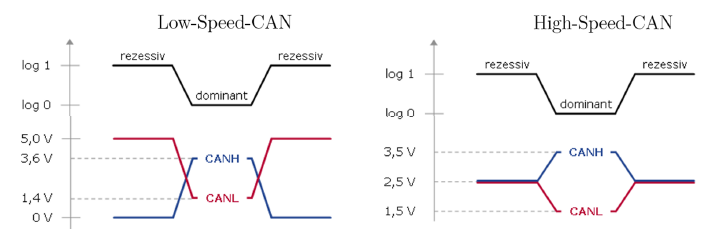
\includegraphics[width=\textwidth]{./2_2_3_Signalpegel-CAN}
	\caption{Signalpegel Low-Speed-\acs{CAN} (links) und High-Speed-\acs{CAN} (rechts) \cite{VectorInformatikGmbH.}.}
	\label{abb:CANSignalpegel}
\end{figure}

\subsection{CAN-Protokoll: Data Link Layer} \label{subsec:DataLinkLayer}
Der \emph{Data Link Layer} beschreibt das Zugriffsverfahren und den strukturellen Aufbau eines \acs{CAN}-\emph{Frames}. Unter einem Frame versteht man den gesamten Datenrahmen, der in einer einzelnen Botschaft über den \acs{CAN}-Bus übermittelt wird. Zwischen den Begriffen Frame, Botschaft und Nachricht wird nachfolgend keine Unterscheidung getroffen. Typischerweise gibt es mehrere Arten von CAN-Frames, die in verschiedene Kategorien unterteilt werden:

\begin{itemize}
	\item \emph{Data Frame} zur Übertragung von Nutzdaten.
	\item \emph{Remote Frame} zur Anforderung von Nutzdaten (also Data Frames) von beliebigen CAN-Knoten. Setzt sich bis auf das fehlende Data Field wie ein Data Frame zusammen.
	\item \emph{Error Frame} zur Signalisierung entdeckter Fehler während des Kommunikationsbetriebs. Mit dem Übertragen eines Error Frames geht der Abbruch der laufenden Botschaftsübertragung einher.
\end{itemize} 

Das Botschaftenformat eines Data Frames ist in Abbildung \ref{abb:CANDataFrame} dargestellt \cite{VectorInformatikGmbH.}. Die einzelnen Komponenten und deren Aufgaben werden nachstehend in der zugehörigen Tabelle \ref{tab:CAN-Data-Frame} näher erklärt.

\begin{figure}[!htbp]
	\centering
	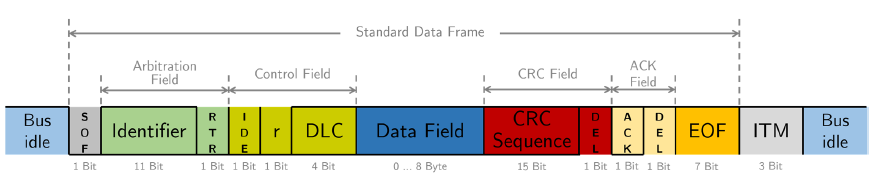
\includegraphics[width=\textwidth]{./2_2_4_CAN-Standard_Data_Frame}
	\caption{Aufbau des Standard \acs{CAN} Data-Frames \cite{VectorInformatikGmbH.}.}
	\label{abb:CANDataFrame}
\end{figure}

\begin{table}[!htbp]
	\centering
	\caption{Funktionen der einzelnen Felder im Data-Frame \cite{Wallentowitz.2011, Zimmermann.2014}.}
	\footnotesize
	\renewcommand{\arraystretch}{1.3}
	\begin{tabular}{l | l l p{7.5cm}}
		\toprule
		Feld              & Name       & Länge       & Funktion                                                                                                                                                                                                          \\ \midrule
		kein Feld         & SOF        & 1 Bit       & Der dominante \emph{Start of Frame} signalisiert den Start eines Frames. Durch den Wechsel von einem rezessiven (Buspegel im Ruhezustand) auf ein dominantes Bit findet eine netzwerkweite Synchronisation statt. \\
		\midrule
		Arbitration Field & Identifier & 11 Bits     & Der Identifier dient der bitweisen Arbitrierung und beschreibt die logische Adressierung der Botschaft.                                                                                                           \\
		                  & RTR        & 1 Bit       & Der \emph{Remote Transmission Request} kennzeichnet	den Frametyp. Im Fall des Data Frames wird das Bit dominant übertragen.                                                                                       \\
		\midrule
		Control Field & IDE        & 1 Bit       & Die \emph{Identifier Extension} legt fest, ob der Identifier im Standard-Format (11 Bit) oder im Extended-Format (29 Bit) vorliegt.                                                                               \\
		                  & r          & 1 Bit       & Dieses Bit ist für künftige Erweiterungen reserviert.                                                                                                                                                             \\
		                  & DLC        & 4 Bits      & Der \emph{Data Length Code} übermittelt die Anzahl der nachfolgenden Nutzbytes.                                                                                                                                   \\
		\midrule
		Data Field        & Data Field & 0...64 Bits & Im Datenfeld werden bis zu acht Bytes an Nutzdaten übertragen. Es beinhaltet die zu übermittelnden Signalwerte und Nutzinformationen.                                                                             \\
		\midrule
		CRC-Field         & CRC        & 15 Bits     & Der \emph{Cyclic Redundancy Check} bildet eine Prüfsumme der Nutzdaten und dient der Fehlererkennung bei der Botschaftsübertragung.                                                                               \\
		                  & DEL        & 1 Bit       & Auf das CRC-Feld folgt ein rezessives \emph{Delimiter}-Bit.                                      \\
		\midrule
		ACK-Field         & ACK        & 1 Bit       & Der Sender einer Botschaft setzt das \emph{Acknowledgement}-Bit auf rezessiv, der Empfänger quittiert das korrekte Ergebnis des CRC-Feldes mit einem dominanten Bit.                                              \\
		                  & DEL        & 1 Bit       & Das ACK-Feld wird ebenfalls durch ein \emph{Delimiter}-Bit begrenzt.                                                                                                                                              \\
		\midrule
		kein Feld         & EOF        & 7 Bit       & Der \emph{End of Frame} markiert das Ende einer Botschaft mit sieben rezessiven Bits.                                                                                                                             \\ \bottomrule
	\end{tabular}
	
	\label{tab:CAN-Data-Frame}
\end{table}

Während der gesamten Laufzeit der Netzwerkverbindung senden die Busknoten ihre Botschaften nach dem \emph{Broadcast}-Verfahren unaufgefordert und ereignisgesteuert auf den Bus. Jeder Empfänger einer Botschaft entscheidet, ob der Inhalt relevant ist und er damit die Nachricht auswertet oder ignoriert. Diese \emph{Akzeptanzfilterung} findet auf Basis der inhaltsbasierten Adressierung eines Frames statt. Hierzu kennzeichnet der \emph{Identifier} \acs{ID} den spezifischen Inhalt einer Botschaft. Der Identifier ist in einem herkömmlichen \acs{CAN}-Protokoll 11 Bit lang. Somit lassen sich bis zu $2^{11} = 2.048$ Botschaften eindeutig unterscheiden. Aufgrund der stetig wachsenden Komplexität moderner Busarchitekturen besteht zudem die Möglichkeit, einen Identifier im Extended-Format aufzubauen. Der \acs{ID} umfasst dann 29 Bit, wodurch $2^{29} = 536.870.912$ unterschiedliche Botschaften differenziert werden können.\\
Durch den ereignisgesteuerten Kommunikationsaufbau kann es häufig vorkommen, dass mehrere Busteilnehmer eine Botschaftsübertragung zum gleichen Zeitpunkt beginnen möchten. Da eine Übertragung aber nicht unterbrochen werden kann und oftmals essentielle sicherheitsrelevante Nachrichten unmittelbar mit vergleichsweise marginalen Botschaften versendet werden, ist es von hoher Bedeutung, sämtliche Botschaften mit Prioritäten zu versehen. Es wird das \emph{Carrier Sense Multiple Access with Collision Avoidance} \acs{CSMA/CA}-Verfahren angewendet. Durch eine \emph{bitweise Arbitrierung} wird dafür gesorgt, dass bei einer Kollision auf dem Bus die Botschaft mit der höchsten Priorität weiterhin übertragen wird. Die höchst priorisierte Botschaft weist immer den niedrigsten nominellen \acs{ID} auf. Durch den Vergleich der dominanten und rezessiven Buspegel ist jeder Knoten darüber informiert, welche Botschaft gerade auf dem Bus übertragen wird. Stellt ein Knoten der aktuell sendet fest, dass der Pegel auf dem Bus nicht seiner gesendeten Botschaft entspricht, stellt dieser umgehend den Sendevorgang ein. Die Echtzeitfähigkeit des Gesamtsystems wird somit nicht gefährdet und Botschaften mit hoher Priorität bleiben deterministisch. \\
Neben einer korrekten Zugriffsfolge sind besonders die Datensicherung und eine zuverlässige Fehlererkennung von großem Stellenwert. Hierzu kommen Mechanismen wie der \emph{Cyclic Redundancy Check} \acs{CRC}, \emph{Acknowledgement} \acs{ACK} oder \emph{Bitstuffing} zum Einsatz. In der \acs{CRC}-Sequenz wird aus dem Frame ein Polynom gebildet, welches durch Division mit einem Modulo-Operator eine Prüfsumme ergibt. Der Empfänger berechnet bei Erhalt einer Botschaft ebenfalls eine \acs{CRC}-Prüfsumme. Stimmen die erhaltenen und berechneten Sequenzen überein, war der strukturelle Aufbau der Botschaftsübertragung korrekt. Mindestens ein Empfänger bestätigt den positiven Erhalt, indem er das \acs{ACK}-Bit auf einen dominanten Pegel setzt. Liegt ein \acs{ACK}-Fehler vor, wurde also entweder vom Sender ein Fehler verursacht oder es befinden sich keine weiteren Teilnehmer am Bus.\\
Die Bitstuffing-Methodik dient der zeitlichen Nachsynchronisation während der Übertragungslaufzeit. Die Synchronisation der Busteilnehmer erfolgt eigentlich über den Flankenwechsel zwischen unterschiedlichen Bits. Liegen jedoch mehrere homogene Bits hintereinander vor, kann diese Synchronisation nicht stattfinden. Um eine korrekte Übertragung zu gewährleisten, fügt der Sender bis zum Ende der \acs{CRC}-Sequenz nach fünf homogenen Bits immer ein komplementäres Bit ein. Der Empfänger entfernt seinerseits diese Stuff-Bits, bevor das empfangene Datenpaket ausgewertet wird. Wird von einem Empfänger eine Folge von mehr als fünf homogenen Bits erkannt, liegt ein Bitstuffing-Fehler vor. Bei der Übertragung eines Data Frames mit 11 Bit Identifier kann der gesamte Botschaftsrahmen also um 29 Bit\footnote{im Worst Case bei acht Datenbytes} auf bis zu 132 Bit anwachsen. \\
Wurde einer der genannten Fehler erkannt, wird ein Fehlersignal gesetzt, welches aus sechs dominanten Bits besteht und damit bewusst gegen die Bitstuffing-Regel verstößt. In diesem Fall wird ein aktives \emph{Error Flag} in einem Error Frame von dem Knoten versendet, welcher den Sendefehler zuerst detektiert hat. Die beteiligten \acs{CAN}-Knoten stellen den Sendevorgang umgehend ein. Wird ein Fehler eines Knoten mehrfach detektiert, kann diesem das Senden verweigert werden. Zur Sicherstellung der systemweiten Datenkonsistenz und zur Reduzierung der Busauslastung kann ein fehlerhafter Knoten vollständig von der Buskommunikation ausgeschlossen werden \cite{Wallentowitz.2011, Zimmermann.2014, VectorInformatikGmbH.}.


\section{Hilfsmittel} \label{sec:Hilfsmittel} %Vector CAnoe, CANcaseXL, ...
In diesem Abschnitt werden die wichtigsten Hilfsmittel vorgestellt, die während der Erstellung der vorliegenden Arbeit und den nachfolgend beschriebenen Abschnitten genutzt wurden.

\subsection{Vector CANoe} \label{subsec:CANoe}
\emph{CANoe} ist ein vielseitiges Software-Werkzeug der Firma \emph{Vector Informatik GmbH}. Es bedient Anwendungsgebiete wie Analyse, Diagnose, Simulation, Stimulation und Test während dem gesamten Entwicklungsprozess von Steuergeräten und Netzwerken. CANoe unterstützt dabei sämtliche gängigen Bussysteme sowie die normierten Transport- und Diagnoseprotokolle. Neben der Überwachung des realen Busverkehrs bietet die Software die Möglichkeit, einfache Teilsysteme bis hin zu komplexen Restbussystemen zu simulieren. Dabei kann die Buskommunikation jederzeit textuell dargestellt und die Signale visuell veranschaulicht werden \cite{VectorInformatikGmbH.2018}.\\
Das Softwaretool liefert zusätzlich die integrierte und firmeneigene Programmiersprache \emph{Communication Access Programming Language} \acs{CAPL}.Die auf \emph{C} basierte Sprache wurde speziell für die Anforderungen zur Entwicklung von Bussystemen angepasst. \acs{CAPL} bietet als eventorientierte Skriptsprache die Möglichkeit, bequem auf Signale zuzugreifen und die Signalwerte zu verändern. Es steht eine Vielzahl an vordefinierter Funktionen zur Verfügung. Ebenso können eigene grafische Benutzeroberflächen erstellt werden, wodurch komplexe Simulationsumgebungen erleichtert werden \cite{VectorInformatikGmbH.07.08.2017}.

\subsection{Vector CANcaseXL} \label{subsec.CANcaseXL}
Das \emph{CANcaseXL} der Firma \emph{Vector Informatik GmbH} ist ein USB-Interface, das eine physikalische Ankopplung eines Computers mit der Software CANoe an ein reales Bussystem erlaubt. Mithilfe dieser Ankopplung ist es möglich, sowohl Busbotschaften zu generieren und diese auf den Bus zu senden, als auch reale Botschaften von angekoppelten Systemen zu auszulesen und auszuwerten. Über die beiden D-Sub Anschlüsse ist eine Verbindung zu \acs{CAN}- oder LIN-Netzwerken realisierbar. Zwar wurde das CANcaseXL inzwischen von neueren Modulen abgelöst und bietet lediglich einen eingeschränkten Funktionsumfang gegenüber der weiteren Produktpalette der \emph{Vector Informatik GmbH}, jedoch eignet es sich aufgrund der vergleichsweise kompakten Bauform besonders für die in dieser Arbeit beschriebenen Anwendung. Zudem ist der integrierte Funktionsumfang für den Einsatz als \acs{CAN}-Interface völlig ausreichend \cite{VectorInformatikGmbH.2015}.





	
%-------------------------------------------------------------------
%  HAUPTTEIL
%-------------------------------------------------------------------
%
	\chapter{Ausgangssituation} 	\label{cha:Ausgangssituation}
\section{Hardware}				\label{sec:EVObotHardware}
\lipsum[1-1]	
\section{Software}				\label{sec:EVObotSoftware}
\lipsum[1-1]
\section{Sensorik}				\label{sec:EVObotSensorik}
\lipsum[1-1]
	
	\chapter{Diagnosesystem} \label{cha:Diagnosesystem}

Dieser Kapitel soll detailliert die zentrale Aufgabe der Arbeit beschreiben. Es solle Verfahren zu Diagnose des EVObots entwickelt und erstellt werden, um im Fahrbetrieb die internen Zustands- und Sensordaten echtzeitnah darzustellen und somit die Applikation des Fahralgorithmus zu erleichtern. 
Zunächst wird die Bedeutung der Diagnose eines komplexen Fahrzeugsystems mit vernetzten Systemen aufgezeigt und ein Konzept zur Fehlerdiagnose am Modellfahrzeug aufgebaut. Nachfolgend wird das Vorgehen und der Aufbau eines Diagnosesystems ausführlich beschrieben. Abschließend wird die Diagnosefunktion validiert und die gewonnen Ergebnisse betrachtet. 

\section{Konzept der Fehlerdiagnose} \label{sec.KonzeptDiagnose} % Allgemeines zur Diagnose im Fzg usw., Methodenauswahl: Warum CAN, Alternativen beschreiben (kabellos?), Use-Case-Diagramm

Aktuelle Fahrzeugsystemen sollten selbstredend stets fehlerfrei und ohne Probleme agieren und die vom Fahrer gewünschten Funktionen vollständig umsetzten. Trotzdem kann es unter gewissen Umständen und äußeren Voraussetzung zu einem Fehlverhalten kommen. Ein Fehler kann im Betrieb eines mechatronischen Systemverbund sowohl mechanisch, elektronisch, als auch softwareseitig auftreten. Durch den stetigen Anstieg des Softwareanteils und der sicherheitskritischen Prozesse im automotiven Bereich steigt die Gefahr eines Softwarefehlers oder einer Software-Anomalie. Ein Fehler wird dabei allgemein nach \emph{EN ISO 9000:2005} \cite{DINDeutschesInstitutfurNormunge.V..201511} als \glqq Nichterfüllung einer Anforderung\grqq{} oder nach \emph{DIN 55350} \cite{DINDeutschesInstitutfurNormunge.V..200805} genauer als \glqq eine unzulässige Abweichung eines Merkmals von einer vorgegebenen Forderung\grqq{} beschrieben. \\
Ein Softwarefehler lässt sich allgemeingültig entweder durch physikalische beziehungsweise chemische Effekte oder durch menschliche Fehlermechanismen wie Denkfehler, Verständnisfehler, Interpretationsfehler oder simple Tippfehler beschreiben. Dabei kann man diese Beschreibung eines Fehlers grundsätzlich in zwei Kategorien einordnen: Man spricht von einem physikalischen Fehler, wenn einzelne Komponenten oder Teilsysteme ausfallen, oder von einem funktionalen Fehler, wenn ein System ausführbar ist, seine Funktion aber nicht korrekt umgesetzt wird \cite{Borcsok.2007}. Ein funktionaler Fehler ist offenbar in den meisten Fällen das Ergebnis von Design-Mängeln und demnach auf eine menschliche Ursache zurückzuführen. Eine Fehlhandlung in der Umsetzung einer Softwareanwendung führt in aller Regel zu einem Fehlerzustand bei der Programmausführung. Dieser Fehlerzustand kann unter Umständen auch unerkannt bleiben. Tritt der Fehlerzustand jedoch aus Programmsicht nach Außen auf, spricht man von der Fehlerwirkung, die für den Anwender wahrnehmbar ist. Diese Fehlerwirkung kann sich je nach Schwere des Fehlers als ein abweichender Rückgabewert einer Berechnung oder bis hin zum Totalausfall des Systems äußern \cite{ISTQBAISBLGermanTestingBoarde.V.2017}. \\
Im Sinne der Zuverlässigkeit gilt es also, das Auftreten eines Fehlerzustandes in einem sicherheitskritischen System zu vermeiden oder besser einen sicheren Zustand im Fehlerfall einzunehmen. Ein übergeordnetes Beispiel eines \emph{Fail-Safe}-Zustandes kann aus der Technologie des hochautomatisierten Fahrens gegeben werden: Fällt das Kamerasystem zur Fahrspurerkennung unerwartet aus, soll ein automatisiert fahrendes Fahrzeug nicht unkontrolliert weiterfahren, sondern die Fahrgeschwindigkeit reduzieren und auf Basis der verfügbaren Streckendaten am rechten Fahrbahnrand zum Stehen kommen, um einen potentiellen Schaden zu minimieren. 

Die Komplexität der vernetzten Funktionen und Systeme erfordert eine umfassende Kommunikation der Softwarekomponenten und ebenso ausgereifte Methoden zur Diagnose möglicher Fehler. Kommt es zu einem Fehlerfall oder Systemausfall, ist die Ursache in einem komplexen und verteilten Systemnetzwerk meist schwer auszumachen. Aufgrund dessen wurden bereits früh in der Entwicklung elektronischer Datenkommunikation Diagnosesysteme als Analysewerkzeug eingeführt. Mit einem aus Hard- und Software bestehenden Diagnosesystem kann die Datenbuskommunikation aufgezeichnet und diagnoserelevante Informationen über den Zustand der Teilkomponenten zu einem externen Testgerät übertragen und ausgewertet werden. Ein Diagnosesystem gilt damit als umfangreiches Werkzeug zur schnellen Fehlererkennung und Fehleranalyse. Während dem Entwicklungsprozess lässt sich ein Diagnosesystem auch nutzen, um über die Diagnosekommunikation die Steuergeräte-Applikation durchzuführen. Dabei ist es nicht nur nötig die reine Datenübertragung einheitlich zu standardisieren, sondern ebenfalls die Applikationsschicht der Protokolle (Vgl. Tabelle \ref{tab:OSI-Schichtenmodell}) zu normieren. Dies bietet die Möglichkeit, den Aufwand und die Pflege der Diagnoseschnittstellen und den Diagnosetestern zu begrenzen. \\
Um eine einheitliche Diagnosekommunikation zu schaffen, wurden seit den 1990er Jahren diverse \emph{Diagnoseprotokolle} entwickelt, die zunächst teils proprietär und inkompatibel zueinander umgesetzt waren, inzwischen jedoch meist herstellerübergreifend genormt sind. Als heute gängige Diagnoseprotokolle sind das \emph{Keyword 2000 Protokoll} \acs{KWP} 2000, die \emph{Unified Diagnostic Services} \acs{UDS} oder die \emph{On-Board-Diagnose} \acs{OBD} zu nennen. Für weiterführende Informationen der genannten Standards sei auf \cite{Zimmermann.2014} und \cite{Schaffer.2012} verwiesen.

\subsection{Anforderungen an die Fehlerdiagnose}
\label{subsec:AnforderungenDiagnose}

Um ein Diagnosesystem für das Demonstratorfahrzeug mit angemessenen Mitteln und Werkzeugen umzusetzen, wird zunächst der gewünschte Funktionsumfang beschrieben und darauf aufbauend sämtliche Anforderungen an das System definiert.
Dazu ist in Abbildung \ref{abb:UseCaseDiagnose} ein Use-Case-Diagramm in der grafischen Modellierungssprache \acs{UML} für den konkreten Anwendungsfall der Diagnosefunktion dargestellt. Hieraus lassen sich leicht die Spezifikationen und geforderte Funktionalitäten an die spätere Diagnose ableiten.

\begin{figure}[!htbp]
	\centering
	\begin{tikzpicture}
	\begin{umlsystem}[x=4, fill=red!10]{Diagnosefunktion} 
	
	\umlusecase [x=0.5, y=0,    width=2.5cm] {Diagnose starten/stoppen}
	\umlusecase [x=0,   y=-2,   width=2.5cm] {Diagnosedaten aufzeichnen}
	\umlusecase [x=0.5, y=-4,   width=2.5cm] {Diagnosedaten ausgeben}
	\umlusecase [x=0,   y=-6,   width=2.5cm] {in Klartext darstellen}
	\umlusecase [x=4,   y=-7.5, width=2.5cm] {Signalverlauf darstellen}
	\umlusecase [x=5,   y=-3,   width=2.5cm] {Daten einlesen}
	\umlusecase [x=5.5, y=-1,   width=2.5cm] {Sensordaten einlesen}
	\umlusecase [x=5.5, y=-5,   width=2.5cm] {statische Daten einlesen}
	% \umsusecase Datenanalyse

	\end{umlsystem}
	\umlactor [y=-2] {Anwender}
	\umlactor [x=13, y=-3] {EVObot}
	
	\umlassoc{Anwender}{usecase-1}
	\umlassoc{Anwender}{usecase-2}
	\umlassoc{Anwender}{usecase-3}
	\umlassoc{EVObot}{usecase-6}
	\umlinherit{usecase-4}{usecase-3}
	\umlinherit{usecase-5}{usecase-3}
	\umlinherit{usecase-7}{usecase-6}
	\umlinherit{usecase-8}{usecase-6}
	\umlextend{usecase-6}{usecase-1} 
	
	\end{tikzpicture}
	\caption{Use-Case-Diagramm einer Diagnosefunktion für den Fahrdemonstrator}
	\label{abb:UseCaseDiagnose}
\end{figure}
	
Das Gesamtsystem besteht aus Fahrzeug, Diagnosewerkzeug und Anwender. Aus dem Use-Case-Diagramm ergeben sich die funktionalen Anforderungen wie folgt:

\begin{itemize}
	\item Das Diagnosesystem muss die Diagnosedaten innerhalb der Programmlaufzeit an ein Ausgabegerät übermitteln.
	\item Das Diagnosesystem muss die Diagnosedaten auf einem externen Ausgabegerät darstellen.
	\item Das Diagnosesystem muss die Daten sowohl in Klartext ausgeben, als auch die einzelnen Signalverläufe grafisch darstellen. 
	\item Die Diagnosefunktion muss vom Anwender gestartet und gestoppt werden können.
	\item Das Diagnosesystem darf im inaktiven Zustand keine Daten vom Fahrzeug übertragen, um die Systemauslastung gering zu halten.\\
\end{itemize}


Zudem lassen sich weiterhin folgende, nichtfunktionale Anforderungen stellen:
\begin{itemize}
	\item Die Umsetzung der Datenkommunikation soll dem Vorbild eines realen und aktuellen Kraftfahrzeuges entsprechen.
	\item Die Datenkommunikation darf kabelgebunden oder kabellos stattfinden.
	\item Das Diagnosesystem muss ein echtzeitnahes Daten-Monitoring ermöglichen.
	\item Das Diagnosesystem soll eine übersichtliche Visualisierung für den Anwender bieten. 
	\item Die Einbindung in das bestehende System soll ohne grundlegende Modifikationen in den implementierten Algorithmen möglich sein.
	\item Die Datenkonsistenz und Datensicherung bei der externen Kommunikation muss gewährleistet sein.
	\item Die Diagnosefunktion muss für spätere Ergänzungen erweiterbar sein.
	\item Die Programmierschnittstelle muss offen und modular sein. 
\end{itemize}


\newpage


Echtzeitnah, Livebeurteilung und Aufzeichnung möglich, visuell gut umsetzbar, Aufwand überschaubar, Einbindung in bestehendes System nur durch Erweiterung, vergleichbare Umsetzung wie im Kfz, Datenkonsistenz und Zuverlässigkeit (Sicherheitsaspekte von CAN), kabellos oder kabelgebunden (keine langen Fahrwege), leichte Erweiterung 



--> Anforderungen definieren
--> Möglichkeiten zur Umsetzung (großer Vorteil CANoe vorhanden und kann Inhaus genutzt werden)
--> 

Off-Board-Kommunikation als Diagnose in ISO Schicht 7 geregelt 
 
Generierung von Diagnosedaten ist von Beginn der Entwicklung an essentiell, um spätere Komplexität zu beherrschen. 





Fehler sind üblich in komplexen Systemen. Sollten vermieden werden, kommen aber unter bestimmten Bedingungen und Voraussetzungen vor. Abhängig von Implementierung, Fehlervermeidung usw. Fale-Safe-Zustand. Fehlerzustand, Fehlerwirkung
Wie äußert sich Fehler oder Fehlfunktion? --> unplausibler Signalwert, falscher Wert oder out of range

Abweichung zum SOLL ist nicht unbedingt programmseitiger Fehler, sondern kann aus Logikfunktion des Programmierers folgen. 

\section{Aufbau einer Datenkommunikation auf CAN-Bus} \label{sec:AufbauDatenkommunikation} % HW-Anbindung an CAN-Bus, Arduino/Jetson, Darstellung Übertragung Dummy-Botschaften cansend/candump...

\section{Implementierung der Diagnosefunktion} \label{sec:ImplementierungDiagnose} % SW-seitige Umsetzung inkl. kompletter Programmablaufplan, Funktionen erklären, Gesamtfunktion in ROS, ... 

\section{Ergebnisbetrachtung} \label{sec:ErgebnisDiagnose} % Zeitkritisch? Echtzeit? Dauer der Verarbeitung, Wiederholungsrate der Sensorsignale, Rechenleistung, Synchronisation, ...
\subsection{Test und Validierung} \label{subsec:TestValidierungDiagnose}
\subsection{Mehrwert der Diagnosefunktion} \label{subsec:MehrwertDiagnose}
% Alternative: UDP Das User Datagram Protocol, kurz UDP, ist ein minimales, verbindungsloses Netzwerkprotokoll, das zur Transportschicht der Internetprotokollfamilie gehört. UDP ermöglicht Anwendungen den Versand von Datagrammen in IP-basierten Rechnernetzen. --> Kabellos!




	
	\chapter{Dynamische Längs- und Querregelung} \label{cha:DynamischeRegelung}
\lipsum[1-1]

\section{Umsetzung des Fahralgorithmus} \label{sec:UmsetzungFahralgorithmus} % Wie ist die Regelung aktuell umgesetzt?

\section{Kritische Analyse der implementierten Algorithmen} \label{sec:KritischeAnalyseAlgorithmen} % An welchen Stellen kann verbesserten werden? Ist Regelalgoritmus zielführend? Vor/Nachteile PID-Regler oder Fuzzy-Regler

\section{Optimierung der Regelung} \label{sec:OptimierungRegelung}

\section{Implementierung der optimierten Spurregelung} \label{sec:ImplementierungRegeleung}

\section{Ergebnisbetrachtung} \label{sec:ErgebnisRegelung}
\subsection{Test und Validierung} \label{subsec:TestValidierungRegelung}
\subsection{Mehrwert der optimierten Spurregelung} \label{subsec:MehrwertRegelung}
	
	
%-------------------------------------------------------------------
%  SCHLUSS
%-------------------------------------------------------------------
%
	\chapter{Zusammenfassung und Ausblick} \label{cha:schluss}
\lipsum[1]

\section{Zusammenfassung} \label{sec:zusammenfassung}
\lipsum[1-4]

\section{Ausblick} \label{sec:ausblick}
\lipsum[1-4]
	
	\listoftables
	\addcontentsline{toc}{chapter}{Tabellenverzeichnis}
	
	\listoffigures
	\addcontentsline{toc}{chapter}{Abbildungsverzeichnis}
	
	\bibliography{005_bib/literatur}
	\addcontentsline{toc}{chapter}{Literaturverzeichnis}
	
	
%-------------------------------------------------------------------
%  ANHANG
%-------------------------------------------------------------------
%
	\appendix
	\chapter{Anhang} \label{app:anhang}

\section{Anhang 1} \label{app:anhang_1}

\section{Anhang 2} \label{app:anhang_2}
	
\end{document}
